\newpage
\section{第 01 周}

\subsection{第 3 课 | 数组、链表、跳表}

\subsubsection{脑图}

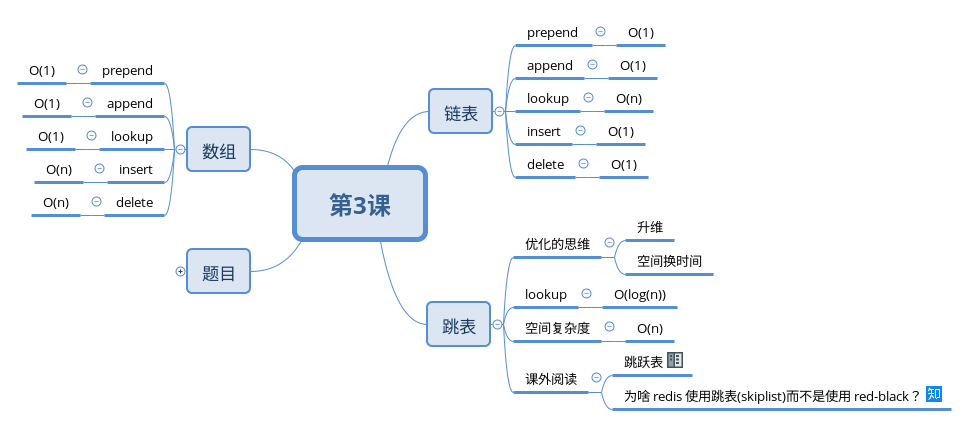
\includegraphics[width=170mm,height=80mm]{images/第3课.png}

\subsubsection{题目}

\paragraph{Array 实战题目}

\begin{itemize}
  \item \hyperref[leetcode:11]{11. 盛最多水的容器}
  \item \hyperref[leetcode:283]{283. 移动零}
  \item \hyperref[leetcode:70]{70. 爬楼梯}
  \item \hyperref[leetcode:15]{15. 三数之和}
\end{itemize}

\paragraph{Link List 实战题目}

\begin{itemize}
  \item \hyperref[leetcode:206]{206. 反转链表}
  \item \hyperref[leetcode:24]{24. 两两交换链表中的节点}
  \item \hyperref[leetcode:141]{141. 环形链表}
  \item \hyperref[leetcode:142]{142. 环形链表 II}
  \item \hyperref[leetcode:25]{25. K 个一组翻转链表}
\end{itemize}

\paragraph{课后作业}

\begin{itemize}
  \item \hyperref[leetcode:26]{26. 删除排序数组中的重复项}
  \item \hyperref[leetcode:189]{189. 旋转数组}
  \item \hyperref[leetcode:21]{21. 合并两个有序链表}
  \item \hyperref[leetcode:88]{88. 合并两个有序数组}
  \item \hyperref[leetcode:1]{1. 两数之和}
  \item \hyperref[leetcode:283]{283. 移动零}
  \item \hyperref[leetcode:66]{66. 加一}
\end{itemize}

\subsection{第 4 课 | 栈、队列、优先队列、双端队列}

\subsubsection{脑图}

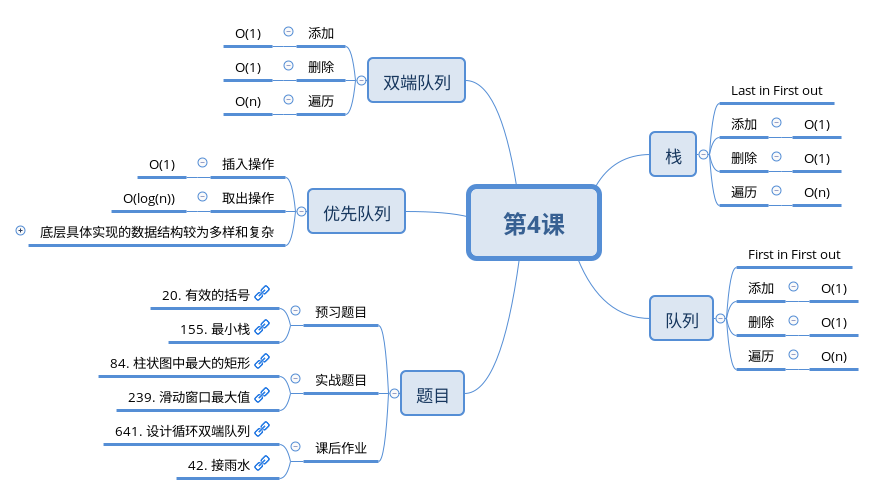
\includegraphics[width=170mm,height=80mm]{images/第4课.png}

\subsubsection{题目}

\paragraph{预习题目}

\begin{itemize}
  \item \hyperref[leetcode:20]{20. 有效的括号}
  \item \hyperref[leetcode:155]{155. 最小栈}
\end{itemize}

\paragraph{实战题目}

\begin{itemize}
  \item \hyperref[leetcode:84]{84. 柱状图中最大的矩形}
  \item \hyperref[leetcode:239]{239. 滑动窗口最大值}
\end{itemize}

\paragraph{课后作业}

\begin{itemize}
  \item \hyperref[leetcode:641]{641. 设计循环双端队列}
  \item \hyperref[leetcode:42]{42. 接雨水}
\end{itemize}


\subsection{学习总结}

这周学习了数组,链表,跳表,栈,队列,
双端队列,优先队列。

数组这个头部插入居然也可以做到 O(1) 的
时间复杂度是我之前没有想到的,但是认真
想下,其实和尾部插入是一样的,都是空间
换时间罢了。

链表这个数据结构最大的弱点就是查找,所以
就出现了跳表这种数据结构。这个优化的过程
用到了升维和空间换时间的思想。链表相关的
题目理解起来没有太多的逻辑困难,但是代码
写起来却很繁琐,很容易出错,需要多多练习。

栈的那些个题目,没有做过的话,都挺难想到
的,像柱状图中最大的矩形,接雨水,都是很
难自己想出来可以使用栈的。

优先队列这个只是一个接口,底层可以用各种
不同的实现方法。你可以用 heap,bst,treap,
甚至你要用数组来实现都是可以的,就是比较慢。

题目分析:盛水最多的容器
这题的双指针向中间靠拢不是很好理解,我这里提供一个思路。

我们把数组最左边的柱子叫做 a,最右边的柱子叫做 b。

假设 a 的高度小于 b。同时在 a 和 b 之间存在着一根柱子 c。

\begin{itemize}
  \item 情况1:c <= a。这种情况 a 和 c 构成的面积一定小于 a 和 b 构成的面积。
  \item 情况2:a < c <= b。这种情况 a 和 c 构成的面积也一定小于 a 和 b 构成的面积。
  \item 情况3:b < c。这种情况 a 和 c 构成的面积还是一定小于 a 和 b 构成的面积。
\end{itemize}

上面 3 种情况,大家自己画个图就清楚了。
你会发现无论 c 是多高的。a 和 c 的面积都不可能
超过 a 和 b 的面积,也就是说柱子 a 和 ab 之间
的任意一根柱子都没有必要判断了。
